\section{Ejercicio 7}

%\subsection{Conclusiones preliminares}
%\begin{itemize}
%	\item Para todos los experimentos existe un quantum a partir del cual aumentarlo no cambia la performance del sistema.
%	\item Para la métrica CPU utilization (que mide la cantidad de tiempo que el CPU está ocupado, entre 0 y 100\% del tiempo, queriendo tenerlo el mayor tiempo ocupado posible), se puede ver con 1 core, que cuando las tareas tienen distinta cantidad de llamadas bloqueantes, el uso del CPU es muy alto, casi 100\%, siendo los ticks de exit de cada tarea al terminar, los únicos que se desperdician. Es decir, se utiliza el CPU durante \textit{cantidad\_total\_de\_ticks - cantidad\_de\_tareas}. Se ve en \textit{ejercicio7\_1core\_quantumX.png} y se estabiliza a partir del test que tiene quantum 8.
%\end{itemize}

Para la resolución de este ejercicio debimos elegir al menos 2 métricas para evaluar la performance de nuestro algoritmo \textit{Round Robin}. A continuación, nuestra experimentación y sus resultados.

\subsection{CPU Utilization}

Para evaluar la performance de nuestro algoritmo con la métrica de utilización del CPU hicimos tanto pruebas single-core como pruebas multi-core, pero lo que queremos mostrar se ve de manera más clara en las pruebas single-core. Los experimentos fueron los siguientes:

\begin{figure}[h]
	\centering                                                       
	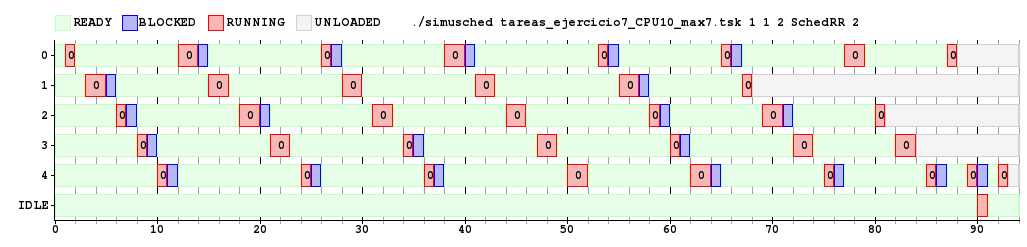
\includegraphics[width=450pt]{./figs/ejercicio7_1core_quantum2.png}
\end{figure}

En la primera prueba, con un quantum de 2 ticks para cada core, podemos ver que la utilización del único CPU disponible es durante un tiempo considerable (poco más de 83\%, siendo lo normal entre 40 y 90\% en un escenario real\footnote{Operating System Concepts - 7th Edition - página 157}).

\begin{figure}[h]
	\centering                                                       
	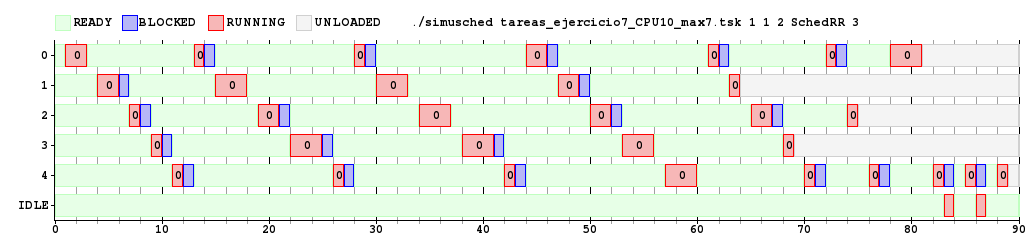
\includegraphics[width=450pt]{./figs/ejercicio7_1core_quantum3.png}
\end{figure}

Aumentando levemente el quantum a 3 ticks por turno, se ve que el \textit{turnaround time}, del cual hablaremos en breve, disminuye, y también el uso del CPU mejora, teniendo menos momentos de CPU en estado ocioso (86$\sim$87\% de tiempo de CPU ocupado).

\begin{figure}[h]
	\centering                                                       
	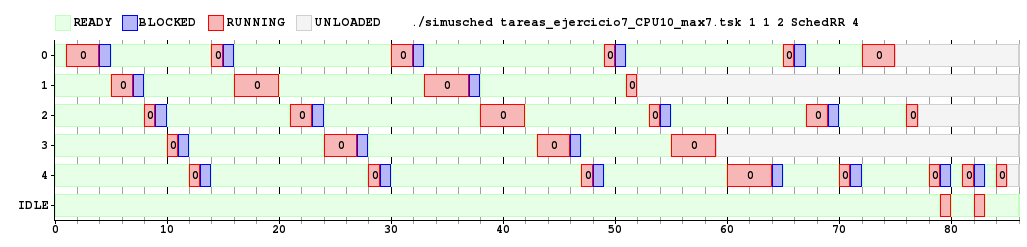
\includegraphics[width=450pt]{./figs/ejercicio7_1core_quantum4.png}
\end{figure}

Con un quantum de 4 ticks, el rendimiento del CPU llega a un 90$\sim$91\%, disminuyendo otra vez el \textit{turnaround time}, pero aumentando el quantum todavía se puede mejorar, como veremos a continuación.

\clearpage

\begin{figure}[h]
	\centering                                                       
	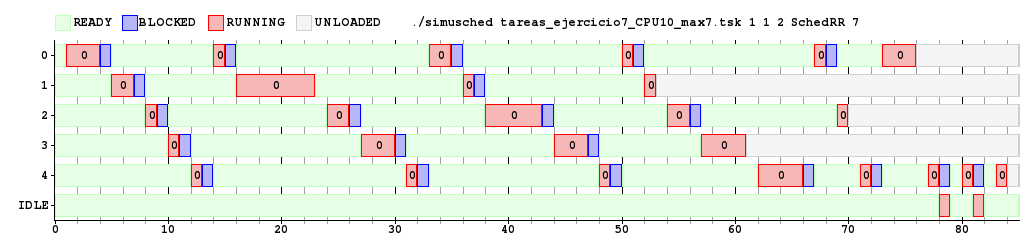
\includegraphics[width=450pt]{./figs/ejercicio7_1core_quantum7.png}
\end{figure}

\begin{figure}[h]
	\centering                                                       
	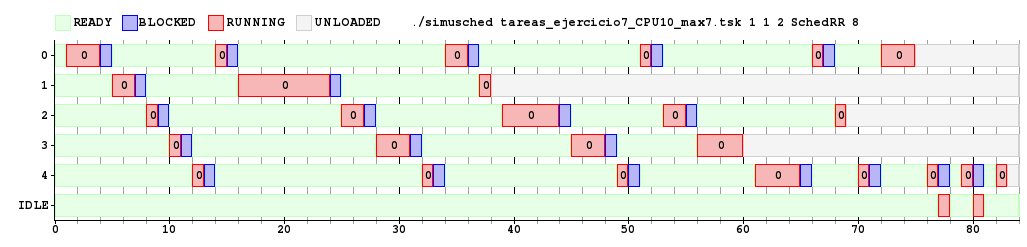
\includegraphics[width=450pt]{./figs/ejercicio7_1core_quantum8.png}
\end{figure}

\begin{figure}[h]
	\centering                                                       
	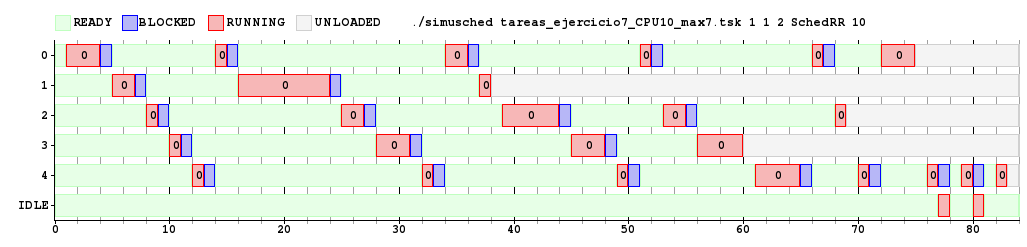
\includegraphics[width=450pt]{./figs/ejercicio7_1core_quantum10.png}
\end{figure}

Hasta un quantum de 7 ticks inclusive, la tarea 1 debe consumir al menos 4 quantums para completarse. A partir de los 8 ticks, en 3 quantums la misma completa su ejecución y termina, disminuyendo drásticamente su \textit{turnaround time}, dado que su \textit{waiting time} se recorta en un turno completo. En el sistema en general, el aumentar el quantum más allá de los 8 ticks por turno ya no mejora la performance del mismo.

\clearpage

\textbf{Perspectiva del core: quantum = 2:}
\begin{figure}[h]
	\centering                                                       
	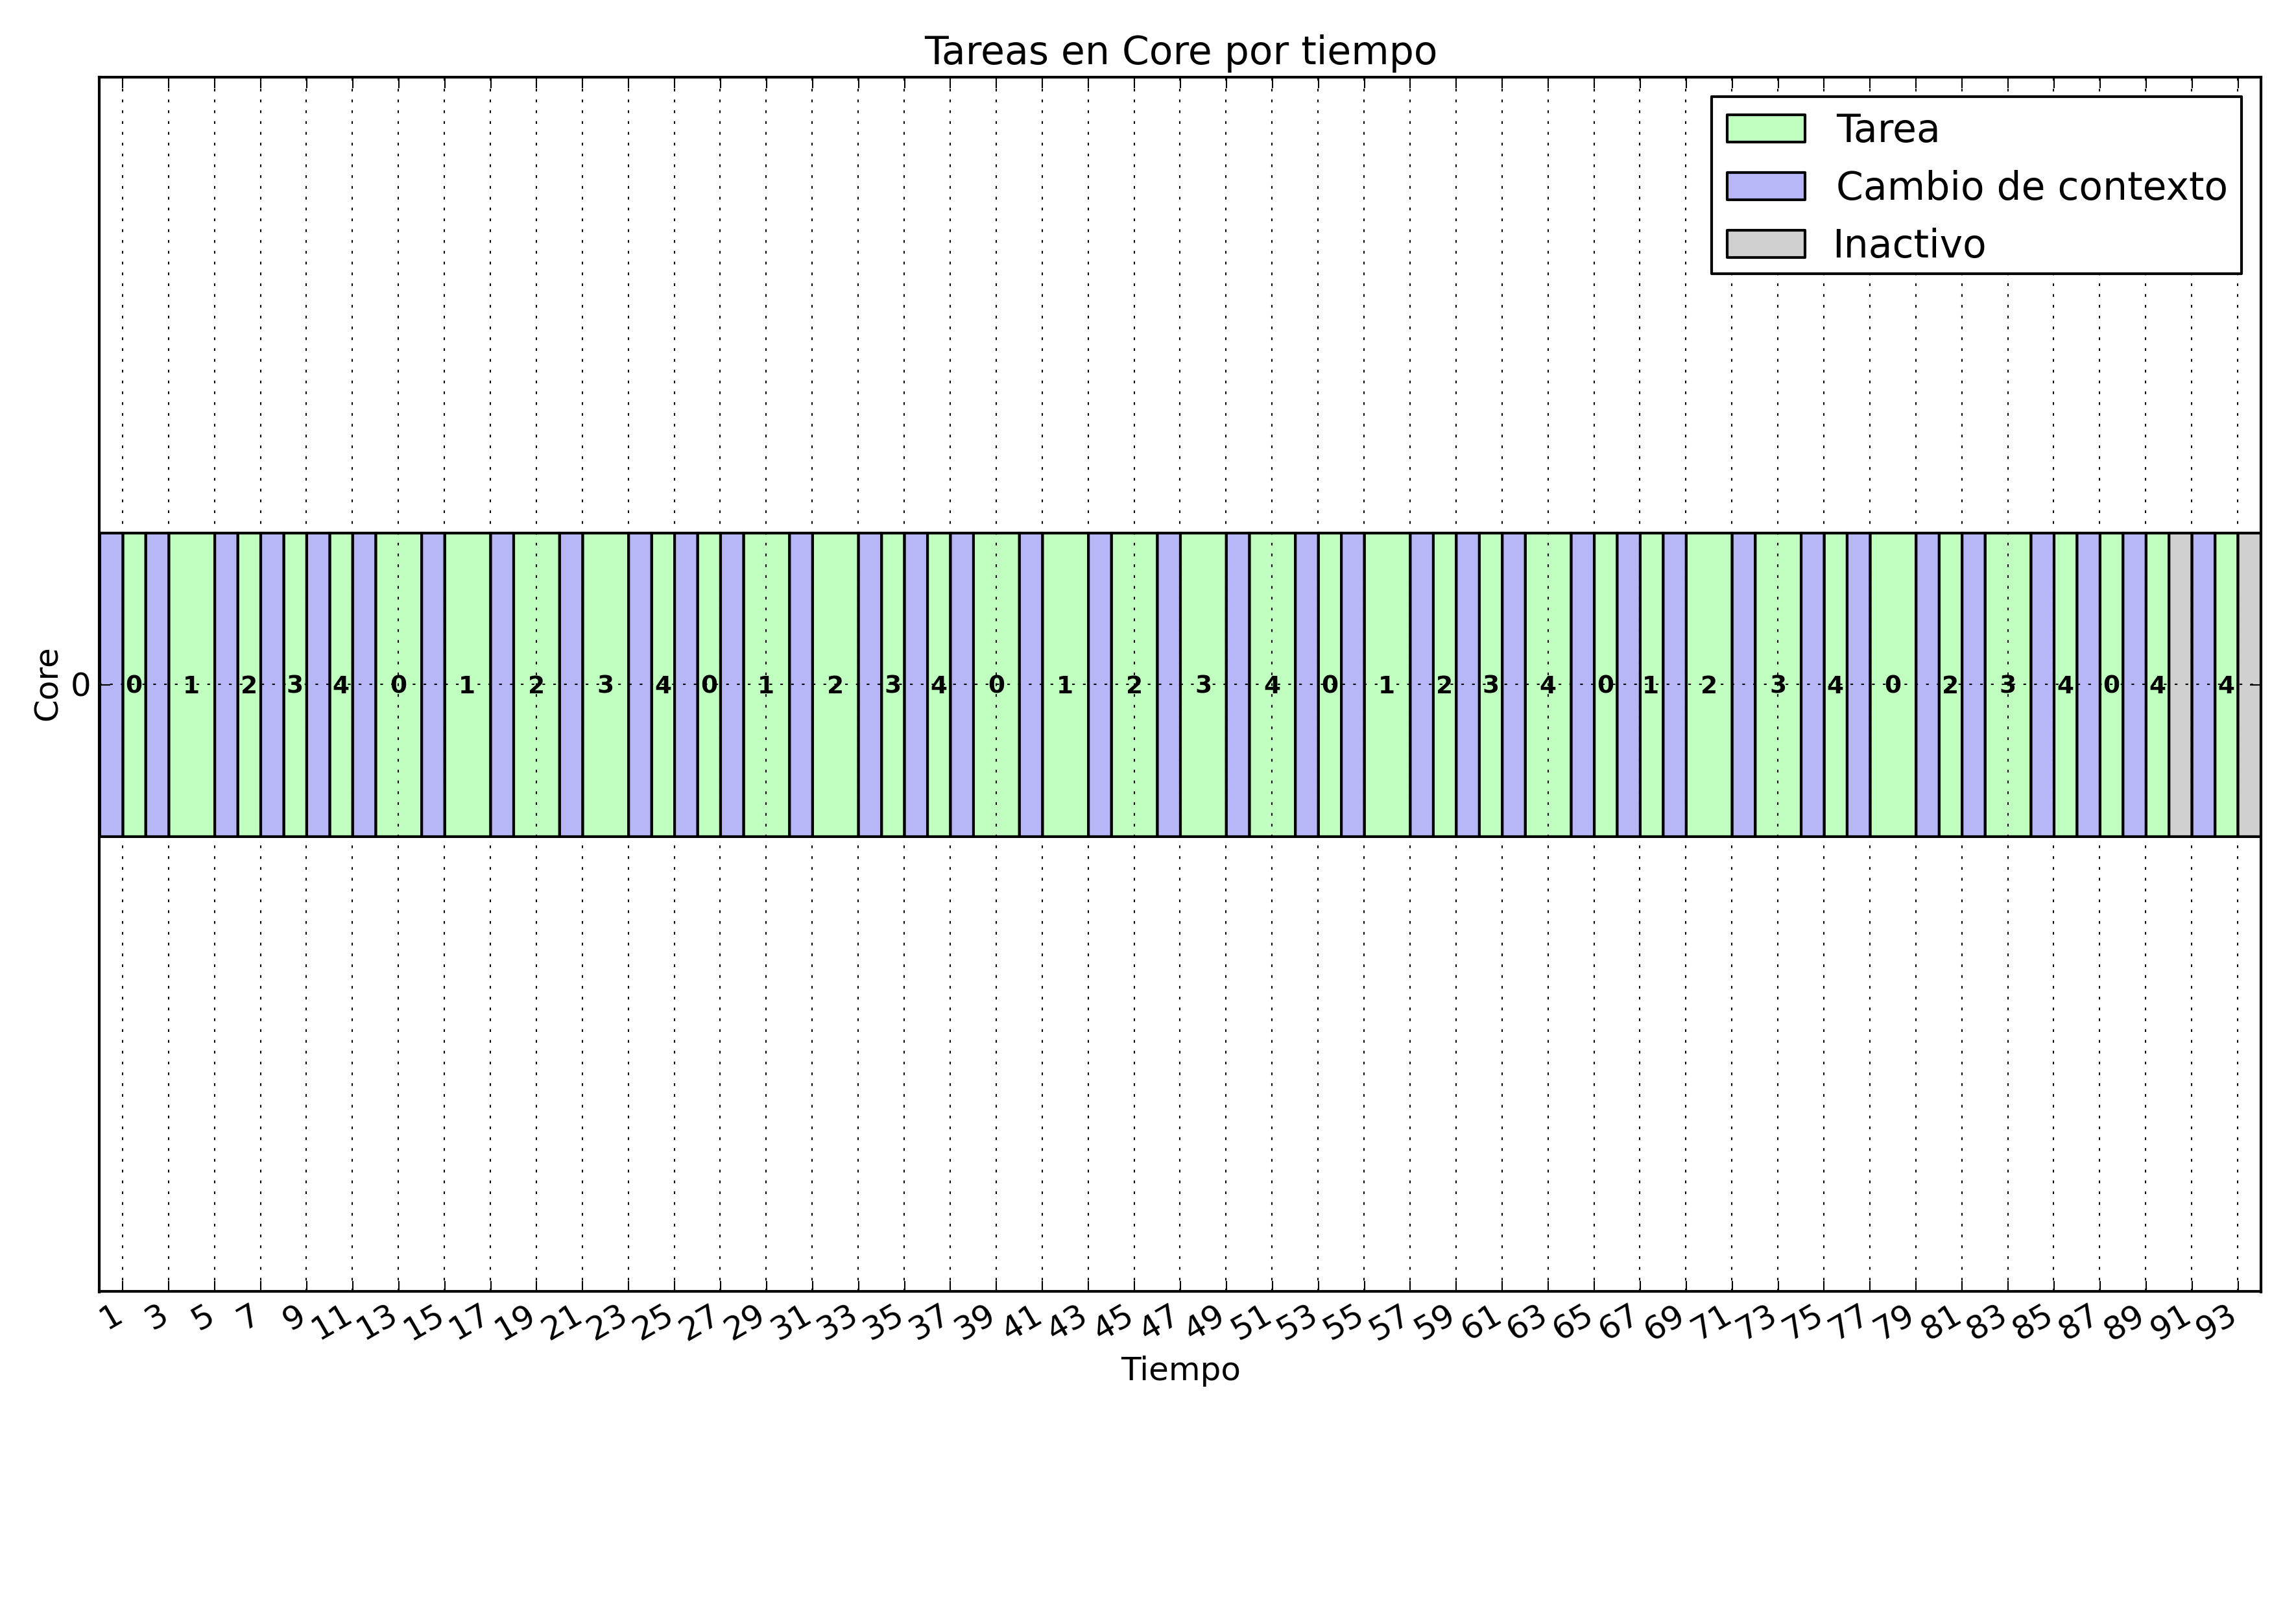
\includegraphics[width=350pt]{./figs/ejercicio7_cores_quantum2.png}
\end{figure}

\textbf{Perspectiva del core: quantum = 10:}
\begin{figure}[h]
	\centering                                                       
	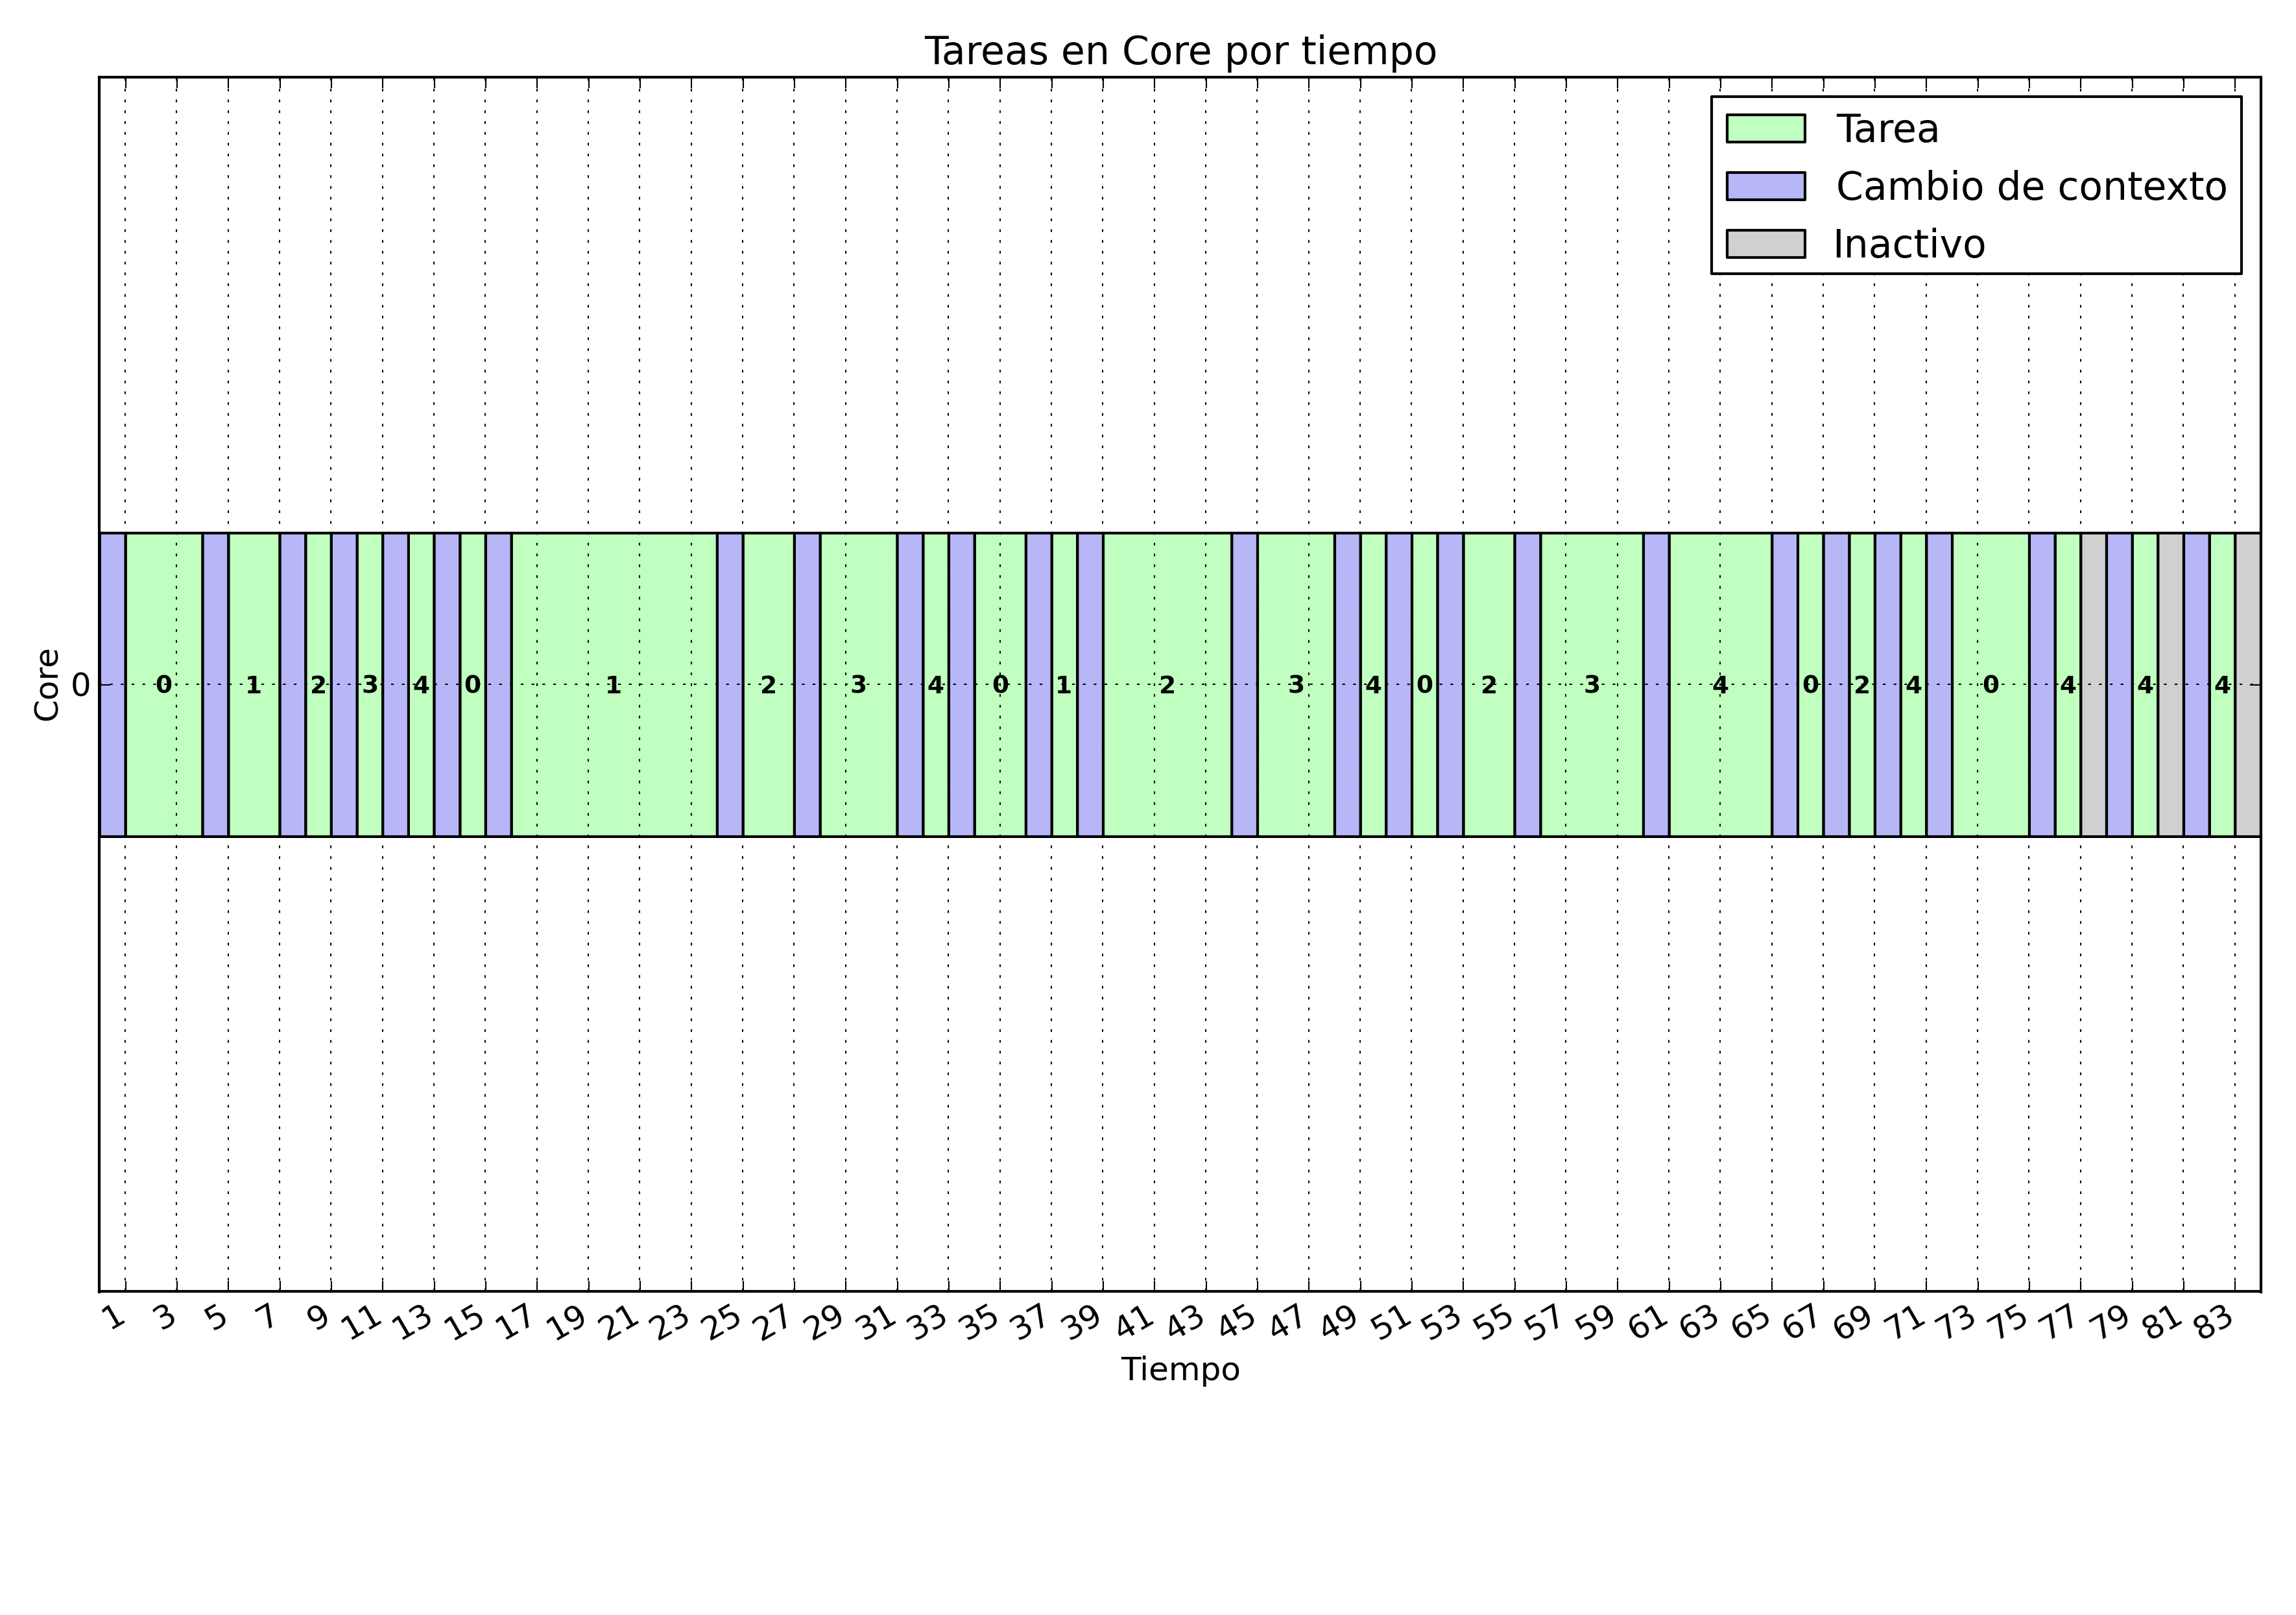
\includegraphics[width=350pt]{./figs/ejercicio7_cores_quantum10.png}
\end{figure}

Para terminar el análisis de este criterio, podemos concluir que el quantum óptimo para este experimento es 8 ticks, y como comentario agregado, podemos decir que se nota la importancia de una buena elección del quantum, viendo que entre el uso de CPU con quantum 2 y el uso con quantum 8, hay una mejora de un 10.63\% aproximadamente.

\subsection{Turnaround time y Waiting time}

Decidimos evaluar el desempeño del algoritmo con los criterios de \textit{turnaround time} y \textit{waiting time} de manera conjunta, ya que creemos que en este tipo de experimentos están íntimamente ligados, al menos en este escenario de prueba. Esto es porque las tareas no son interactivas, en cuyo caso habría que ver también (y por separado) el \textit{response time}, que se encarga de evaluar el tiempo neto utilizado por el CPU una vez que se terminó la interacción con el usuario\footnote{Operating System Concepts - 7th Edition - página 157, 158}, que en general, es órdenes de magnitud más lento que lo que vimos hasta ahora.\\

\textbf{2 cores:}
\begin{figure}[h]
	\centering                                                       
	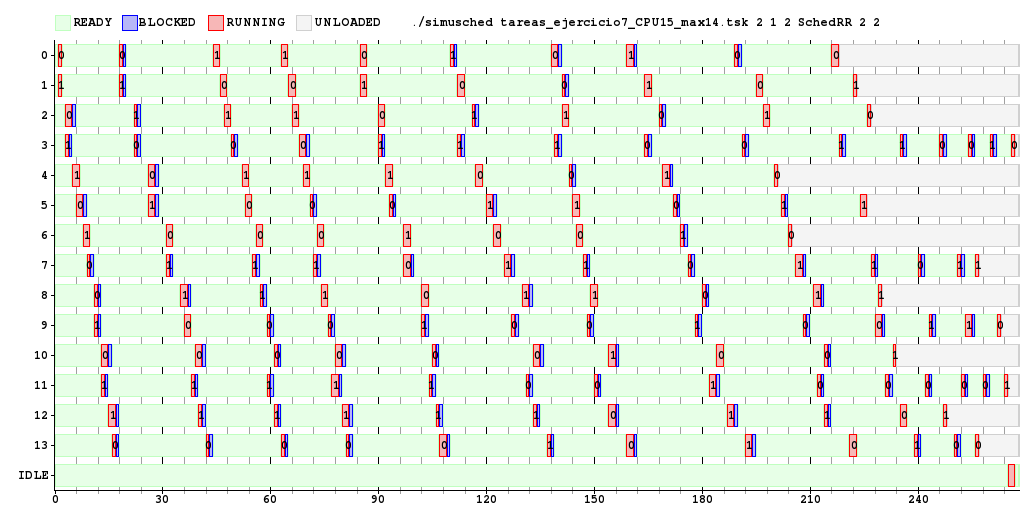
\includegraphics[width=450pt]{./figs/ejercicio7_t15_2cores_quantum2.png}
\end{figure}

\begin{figure}[h]
	\centering                                                       
	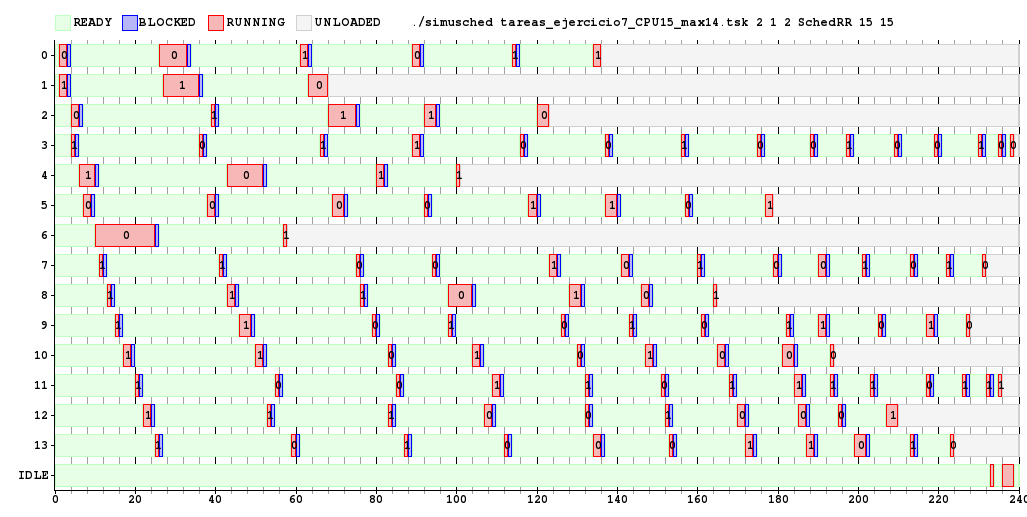
\includegraphics[width=450pt]{./figs/ejercicio7_t15_2cores_quantum15.png}
\end{figure}

En el ejemplo con 2 núcleos se puede ver una mejora sustancial entre un quantum pequeño (2 ticks) y que corta muchas veces la ejecución de cada tarea, contra el quantum óptimo (15 ticks) que interrumpe menos veces la ejecución. Dicha mejora es de alrededor de 24 ticks, o aproximadamente un 10\% menos en el \textit{turnaround time}.\\
\indent Además se puede apreciar como en la mayoría de las tareas, el \textit{waiting time} es drásticamente reducido gracias al aumento del quantum por turno, teniendo hasta 7 turnos menos que ejecutar en casos como la tarea 1 o la 6, reduciendo el \textit{waiting time} de las tareas de manera altamente sustancial, hasta más de 120 ticks en algunos casos como por ejemplo en la tarea 6.

\clearpage

\textbf{3 cores:}
\begin{figure}[h]
	\centering                                                       
	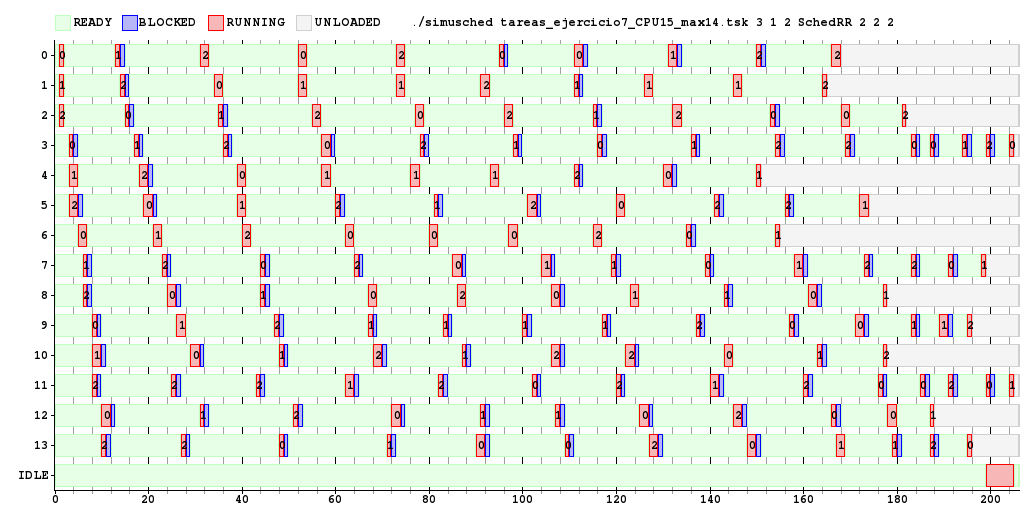
\includegraphics[width=450pt]{./figs/ejercicio7_t15_3cores_quantum2.png}
\end{figure}

\begin{figure}[h]
	\centering                                                       
	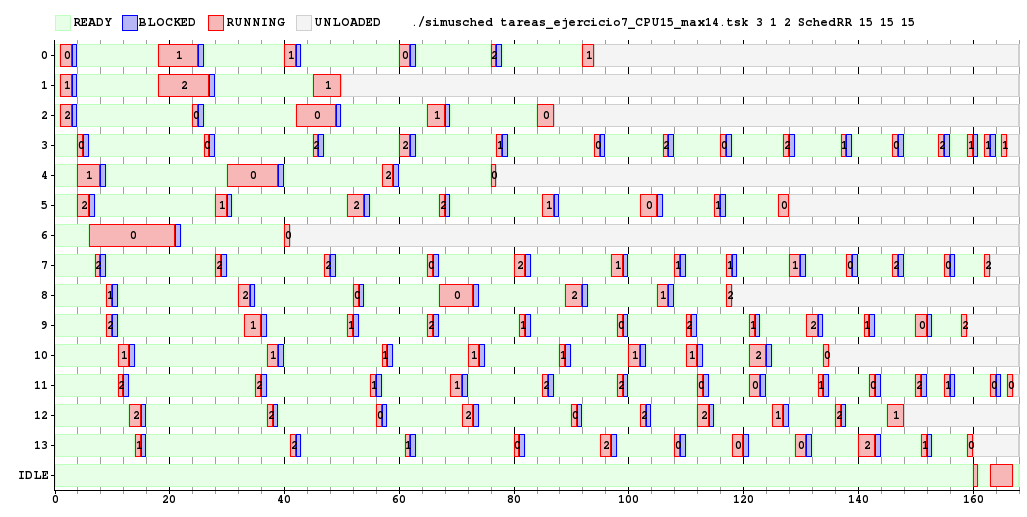
\includegraphics[width=450pt]{./figs/ejercicio7_t15_3cores_quantum15.png}
\end{figure}

\clearpage

\textbf{4 cores:}
\begin{figure}[h]
	\centering                                                       
	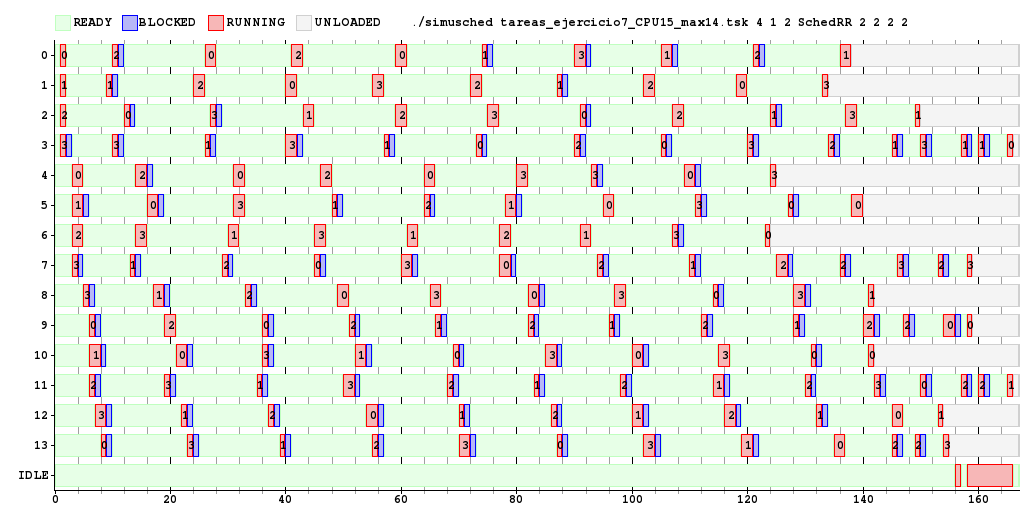
\includegraphics[width=450pt]{./figs/ejercicio7_t15_4cores_quantum2.png}
\end{figure}

\begin{figure}[h]
	\centering                                                       
	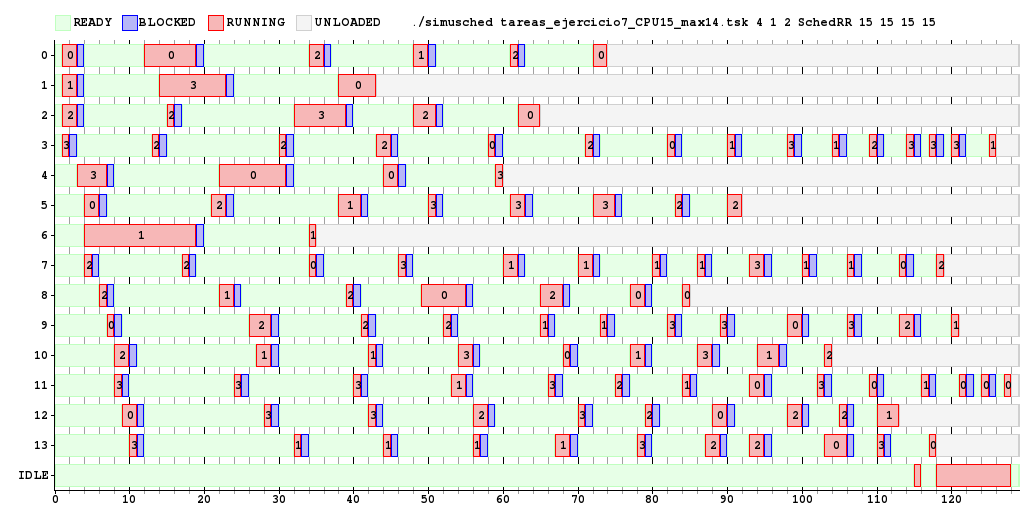
\includegraphics[width=450pt]{./figs/ejercicio7_t15_4cores_quantum15.png}
\end{figure}

Estos comportamientos se ven reflejados de manera similar en los casos con más cores (en este caso mostramos los casos de 3 y 4 cores), siendo la disminución del \textit{waiting time} proporcional a la disminución del \textit{turnaround time} total, gracias al aumento de \textit{throughput} (cantidad de tareas finalizadas en una unidad de tiempo\footnote{Operating System Concepts - 7th Edition - página 157}) debido al agregado de cores de trabajo.